\documentclass[14pt,a4paper,report]{report}
\usepackage[a4paper, mag=1000, left=2.5cm, right=1cm, top=2cm, bottom=2cm, headsep=0.7cm, footskip=1cm]{geometry}
\usepackage[utf8]{inputenc}
\usepackage[english,russian]{babel}
\usepackage{indentfirst}
\usepackage[dvipsnames]{xcolor}
\usepackage[colorlinks]{hyperref}
\usepackage{listings} 
\usepackage{fancyhdr}
\usepackage{caption}
\usepackage{graphicx}
\hypersetup{
	colorlinks = true,
	linkcolor  = black
}

\usepackage{titlesec}
\titleformat{\chapter}
{\Large\bfseries} % format
{}                % label
{0pt}             % sep
{\huge}           % before-code


\DeclareCaptionFont{white}{\color{white}} 

% Listing description
\usepackage{listings} 
\DeclareCaptionFormat{listing}{\colorbox{gray}{\parbox{\textwidth}{#1#2#3}}}
\captionsetup[lstlisting]{format=listing,labelfont=white,textfont=white}
\lstset{ 
	% Listing settings
	inputencoding = utf8,			
	extendedchars = \true, 
	keepspaces = true, 			  	 % Поддержка кириллицы и пробелов в комментариях
	language = C,            	 	 % Язык программирования (для подсветки)
	basicstyle = \small\sffamily, 	 % Размер и начертание шрифта для подсветки кода
	numbers = left,               	 % Где поставить нумерацию строк (слева\справа)
	numberstyle = \tiny,          	 % Размер шрифта для номеров строк
	stepnumber = 1,               	 % Размер шага между двумя номерами строк
	numbersep = 5pt,              	 % Как далеко отстоят номера строк от подсвечиваемого кода
	backgroundcolor = \color{white}, % Цвет фона подсветки - используем \usepackage{color}
	showspaces = false,           	 % Показывать или нет пробелы специальными отступами
	showstringspaces = false,    	 % Показывать или нет пробелы в строках
	showtabs = false,           	 % Показывать или нет табуляцию в строках
	frame = single,              	 % Рисовать рамку вокруг кода
	tabsize = 2,                  	 % Размер табуляции по умолчанию равен 2 пробелам
	captionpos = t,             	 % Позиция заголовка вверху [t] или внизу [b] 
	breaklines = true,           	 % Автоматически переносить строки (да\нет)
	breakatwhitespace = false,   	 % Переносить строки только если есть пробел
	escapeinside = {\%*}{*)}      	 % Если нужно добавить комментарии в коде
}

\begin{document}

\def\contentsname{Содержание}

% Titlepage
\begin{titlepage}
	\begin{center}
		\textsc{Санкт-Петербургский Политехнический 
			Университет Петра Великого\\[5mm]
			Кафедра компьютерных систем и программных технологий}
		
		\vfill
		
		\textbf{Отчёт по лабораторной работе №2\\[3mm]
			Курс: «Защита информации»\\[6mm]
			Тема: «Исследование сетевого трафика протокола FTP»\\[35mm]
		}
	\end{center}
	
	\hfill
	\begin{minipage}{.5\textwidth}
		Выполнил студент:\\[2mm] 
		Бояркин Никита Сергеевич\\
		Группа: 43501/3\\[5mm]
		
		Проверил:\\[2mm] 
		Новопашенный Андрей Гелиевич
	\end{minipage}
	\vfill
	\begin{center}
		Санкт-Петербург\\ \the\year\ г.
	\end{center}
\end{titlepage}

% Contents
\tableofcontents
\clearpage

\chapter{Лабораторная работа №2}

\section{Цель работы}

Получение навыков по исследованию сетевого трафика.

\section{Программа работы}

При помощи программы WireShark продемонстрировать сетевой трафик для:

\begin{itemize}
	\item Протокола FTP
		\begin{itemize}
			\item В пассивном режиме
			\item В активном режиме
			\item Установление соединения и авторизация
		\end{itemize}
\end{itemize}

\section{Конфигурация сети}

\begin{figure}[h!]
	\centering
	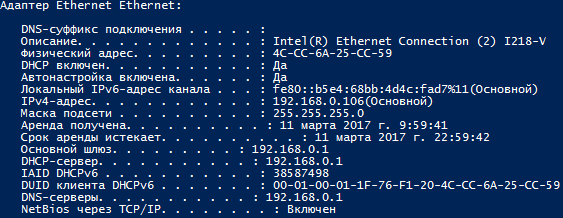
\includegraphics[scale = 1.1]{images/config.png}
	
	\caption{Сетевые параметры компьютера}
	\label{image:1}
\end{figure}

\section{Ход работы}

\subsection{Протокол FTP}

В отличие от большинства других протоколов, при работе с протоколом FTP создается два типа соединений, первое  служит для аутентификации и передачи команд, второе — для передачи данных. По второму соединению определяется режим работы, он может быть активным, а может быть пассивным. Отличаются они между собой стороной выступающей инициатором подключения для передачи данных и портами, на которых эта передача собственно производиться. При нормальном или активном FTP, управляющее соединение инициируется со стороны клиента, а подключение для передачи данных инициируется со стороны сервера. В пассивном режиме, как управляющее соединение так и соединение для передачи данных инициируется клиентом.

Для демонстрации работы протокола FTP был выбран сервер ftp://ftp.funet.fi (193.166.3.2).

\subsection{Установление управляющего соединения}

Первый этап - установление TCP соединения с 21 портом сервера (управляющее соединение):

\begin{figure}[h!]
	\centering
	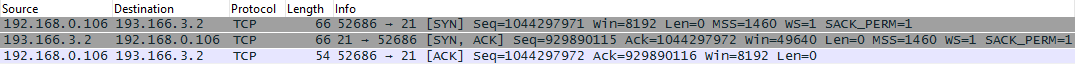
\includegraphics[scale = 0.62]{images/ftp1.png}
	
	\caption{Установление TCP соединения с 21 портом сервера}
	\label{image:3}
\end{figure}

Стандартная процедура проверки достижимости сервера. Применяется для всех протоколов, использующих TCP. Аналогичное установление соединения происходит с потоком данных после аутентификации и перехода в активный/пассивный режим.

\subsection{Аутентификация}

Следующий этап - аутентификация клиента с помощью имени пользователя и пароля. Имя пользователя отправляется на сервер командой USER, а пароль - командой PASS.

Хост, обеспечивающий FTP-сервис, может предоставить анонимный доступ к FTP. Пользователи обычно входят в систему как «anonymous» в качестве имени пользователя. Хотя обычно пользователей просят прислать адрес их электронной почты вместо пароля, никакой проверки фактически не производится. Многие FTP-хосты, предоставляющие обновления программного обеспечения, поддерживают анонимный доступ.

\begin{figure}[h!]
	\centering
	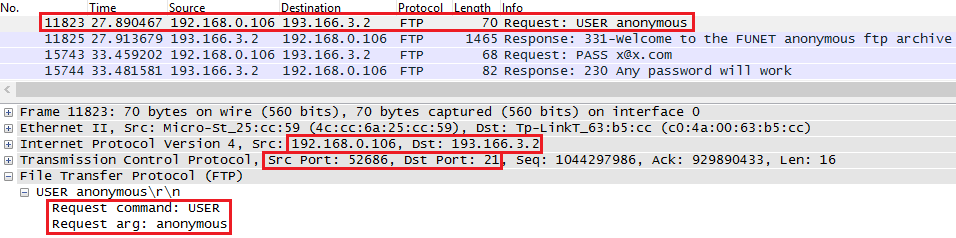
\includegraphics[scale = 0.70]{images/ftp2.png}
	
	\caption{Отправка имени пользователя командой USER}
	\label{image:4}
\end{figure}

\begin{figure}[h!]
	\centering
	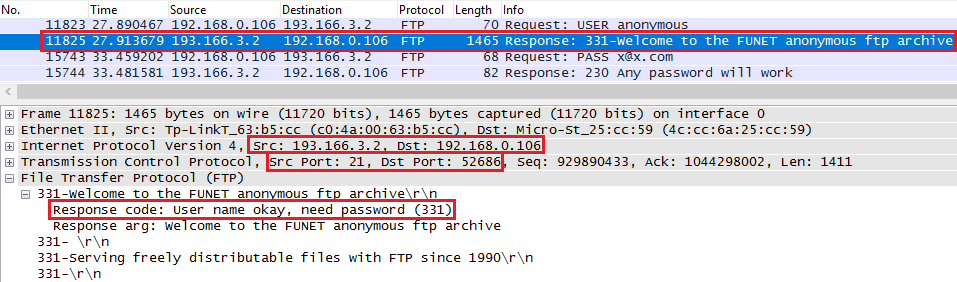
\includegraphics[scale = 0.70]{images/ftp3.png}
	
	\caption{Реакция сервера на правильное имя пользователя}
	\label{image:5}
\end{figure}

Реакция сервера на имя пользователя - это FTP пакет с кодом 331 (имя пользователя корректно). Если имя пользователя не существует, то специальный FTP пакет с кодом ошибки не посылается (только на следующем этапе проверки пары имени пользователя и пароля). Это сделано для того, чтобы клиент не мог определить какие пользователи существуют на сервере.

\clearpage

\begin{figure}[h!]
	\centering
	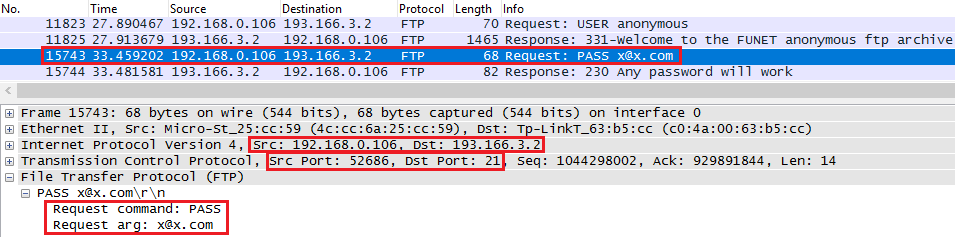
\includegraphics[scale = 0.63]{images/ftp4.png}
	
	\caption{Отправка пароля командой PASS}
	\label{image:6}
\end{figure}

\begin{figure}[h!]
	\centering
	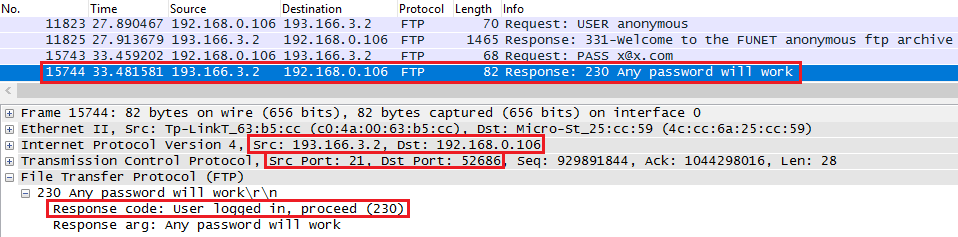
\includegraphics[scale = 0.66]{images/ftp5.png}
	
	\caption{Реакция сервера на правильный пароль}
	\label{image:7}
\end{figure}

Если пара имя пользователь и пароль правильная, то сервер возвращает FTP пакет с кодом 230 (пользователь идентифицирован), если нет, то 530 (вход не выполнен).

Стоит отметить, что ни имя пользователя, ни пароль не зашифровываются.

\subsection{Активный режим FTP}

\begin{figure}[h!]
	\centering
	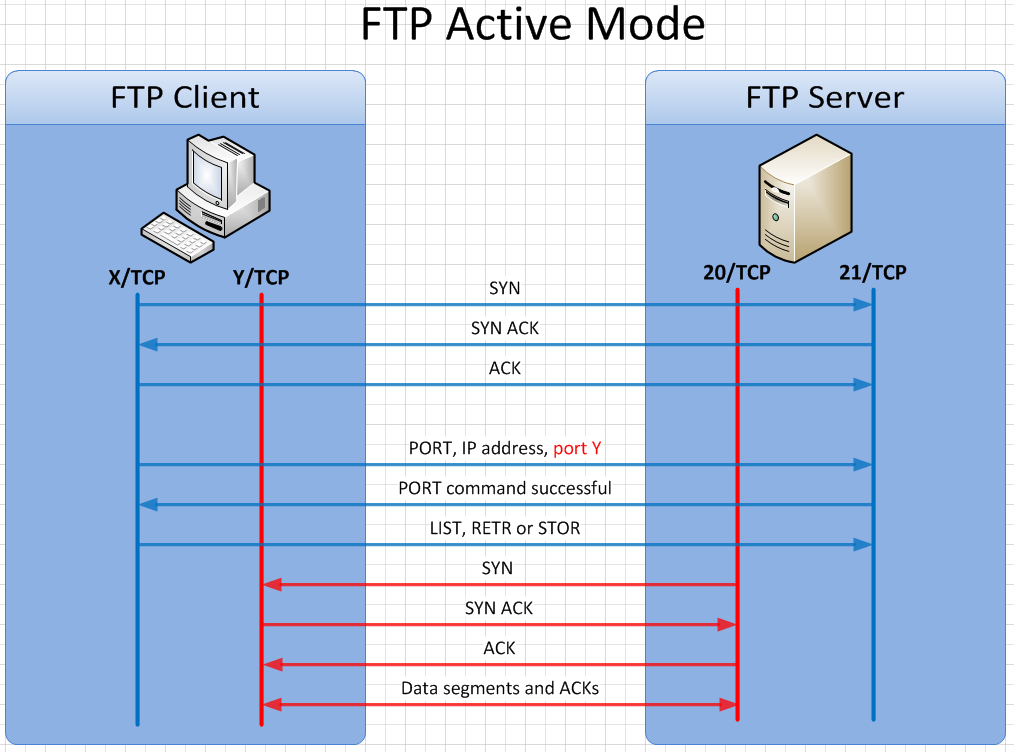
\includegraphics[scale = 0.55]{images/scheme_ftp_active.png}
	
	\caption{Клиент-серверное взаимодействие в активном режиме FTP}
	\label{image:2}
\end{figure}

Для перехода в активный режим клиент явно указывает собственный IP адрес (первые 4 байта аргумента) и порт подключения (последние 2 байта аргумента) командой PORT:

\begin{figure}[h!]
	\centering
	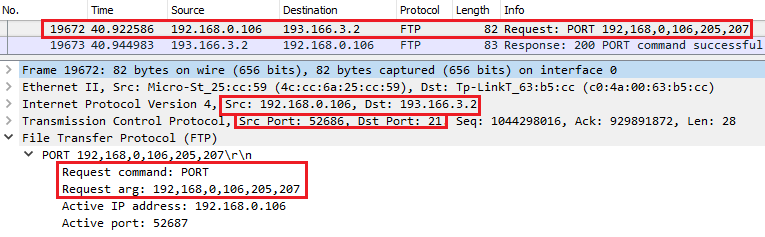
\includegraphics[scale = 0.73]{images/ftp6.png}
	
	\caption{Переход в активный режим}
	\label{image:8}
\end{figure}

\begin{figure}[h!]
	\centering
	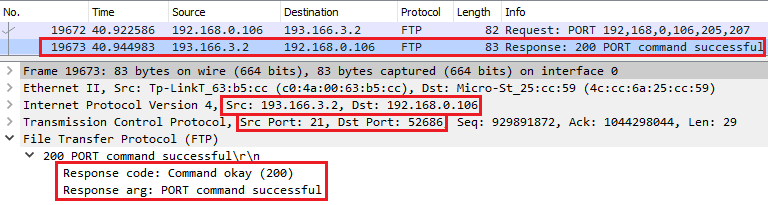
\includegraphics[scale = 0.73]{images/ftp7.png}
	
	\caption{Реакция сервера на успешный переход в активный режим}
	\label{image:9}
\end{figure}

В случае успешного перехода в активный режим сервер возвращает FTP пакет с кодом 200 (команда корректна). После этого становятся доступными команды LIST, PETR, STORE и др. Установление соединения потока данных инициируется со стороны сервера после первой команды от клиента (аналогично уже рассмотренному в п. 1.4.2).

\subsection{Пассивный режим FTP}

\begin{figure}[h!]
	\centering
	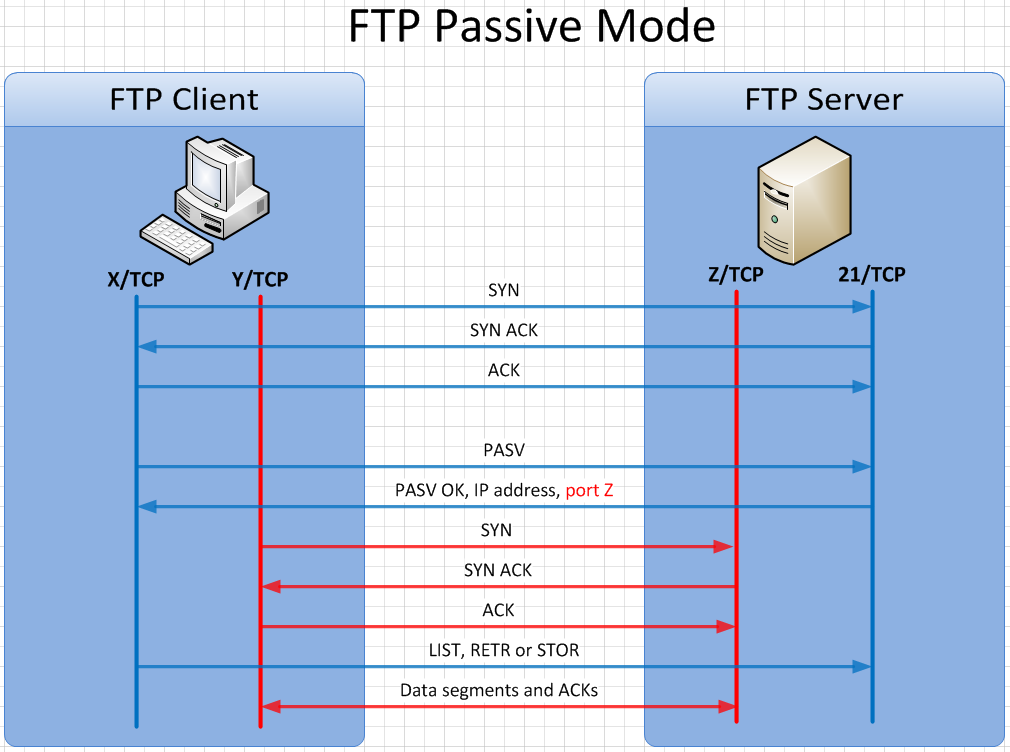
\includegraphics[scale = 0.44]{images/scheme_ftp_passive.png}
	
	\caption{Клиент-серверное взаимодействие в пассивном режиме FTP}
	\label{image:10}
\end{figure}

Для перехода в пассивный режим клиент отправляет на сервер FTP пакет с единственной командой PASV:

\begin{figure}[h!]
	\centering
	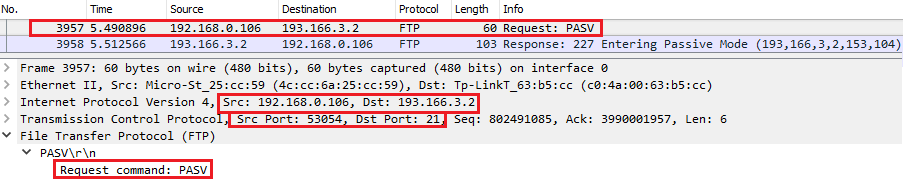
\includegraphics[scale = 0.73]{images/ftp8.png}
	
	\caption{Переход в пассивный режим}
	\label{image:11}
\end{figure}

В ответ сервер посылает FTP пакет с кодом 227 (переход в пассивный режим) и парой значений: IP адрес (первые 4 байта аргумента) и порт подключения (последние 2 байта аргумента): 

\begin{figure}[h!]
	\centering
	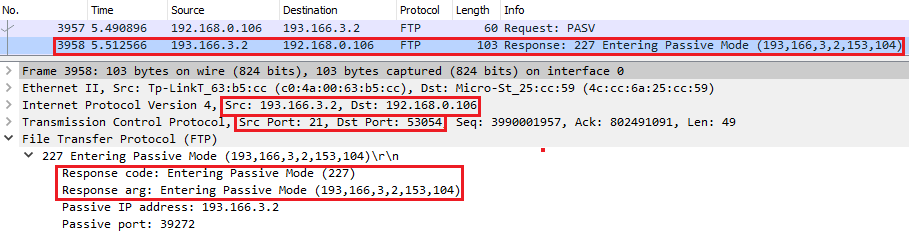
\includegraphics[scale = 0.73]{images/ftp9.png}
	
	\caption{Реакция сервера на успешный переход в пассивный режим}
	\label{image:12}
\end{figure}

После этого клиент инициирует установление соединения потока данных (аналогично уже рассмотренному в п. 1.4.2). После установления соединения потока данных становятся доступными команды LIST, PETR, STORE и др.

\section{Вывод}

В ходе работы был исследован сетевой трафик протокола FTP в активном и пассивном режиме.

Протокол FTP не безопасен, потому что не поддерживает шифрование данных. Это обусловлено том, что во времена создания протокола проблема защиты данных не была так актуальна. Для решения проблемы безопасности были созданы защищенные вариации FTP, такие как:

\begin{itemize}
	\item FTPS
	\item SFTP
	\item FTP через SSH
\end{itemize}
	
В большинстве случаев используется пассивный режим FTP соединения. Это обусловлено тем, что в пассивном режиме все соединения инициирует клиент и поэтому к нему нет никаких требований, он может находиться за NAT и брандмауэром, а также не иметь выделенного IP-адреса.

В активном режиме основная проблема возникает у клиента. Если брандмауэр настроен отбрасывать не инициированные изнутри входящие соединения, то сервер не сможет установить соединение для передачи данных. А так как порт для данных является динамическим, то возникают определенные сложности с настройкой брандмауэра. Наиболее правильным будет указать в клиенте диапазон используемых портов и создать для них разрешающее правило брандмауэра.

\clearpage

\section{Приложение 1. Активный режим FTP}

\subsection{Передача данных}

Рассмотрим процесс передачи данных в активном режиме. В этом режиме мы должны наблюдать, что установление соединения канала данных инициируется сервером с 20 порта (рис 1.7).

Рассмотрим полный процесс получения информации о каталоге (команда LIST):

\begin{figure}[h!]
	\centering
	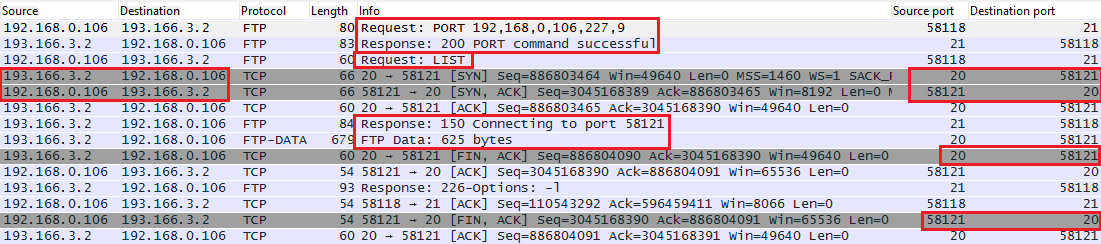
\includegraphics[scale = 0.60]{images/ftp10.png}
	
	\caption{Процесс передачи данных в активном режиме}
	\label{image:15}
\end{figure}

В первую очередь, клиент посылает на сервер (по управляющему каналу) команду PORT с информацией (IP + port) для последующего подключения канала данных. Сервер отвечает кодом 200 (команда успешно выполнена), после чего клиентом отправляется команда LIST. Затем, сервер инициирует установку соединения данных с 20 порта на клиентский порт, указанный в команде PORT ранее. Как только соединение данных установлено, клиенту отправляется сообщение с кодом 150 (подготавливается открытие канала), а также результат операции получения каталога. Финальным этапом является завершение соединения канала данных: клиенту отправляется сообщение с кодом 226 (закрытие канала, обмен завершен успешно), а канал данных обменивается флагами FIN и соединение завершается.

Рассмотрим содержимое этих пакетов подробнее:

\begin{figure}[h!]
	\centering
	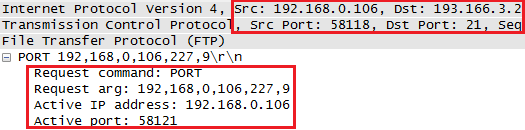
\includegraphics[scale = 0.75]{images/ftp11.png}
	
	\caption{Переход в активный режим}
	\label{image:16}
\end{figure}

\begin{figure}[h!]
	\centering
	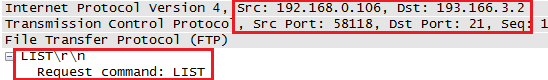
\includegraphics[scale = 0.75]{images/ftp12.png}
	
	\caption{Запрос на получение информации о каталоге}
	\label{image:17}
\end{figure}

\begin{figure}[h!]
	\centering
	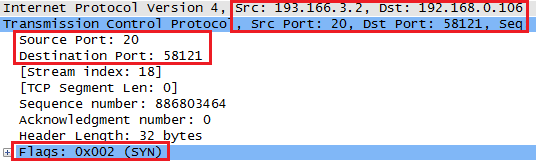
\includegraphics[scale = 0.75]{images/ftp13.png}
	
	\caption{Запрос на установление соединения данных от FTP сервера}
	\label{image:18}
\end{figure}

\clearpage

\begin{figure}[h!]
	\centering
	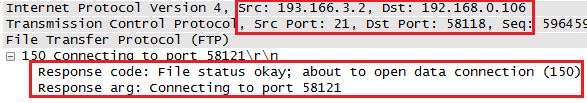
\includegraphics[scale = 0.75]{images/ftp14.png}
	
	\caption{Сообщение об успешном открытии канала данных}
	\label{image:19}
\end{figure}

\begin{figure}[h!]
	\centering
	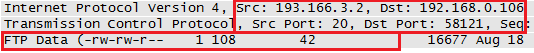
\includegraphics[scale = 0.75]{images/ftp15.png}
	
	\caption{Результат выполнения запрашиваемой команды}
	\label{image:20}
\end{figure}

\section{Приложение 2. Пассивный режим FTP}

\subsection{Передача данных}

Рассмотрим процесс передачи данных в пассивном режиме. В этом режиме мы должны наблюдать, что установление соединения канала данных инициируется клиентом на порт, указанный сервером в ответе на команду PASV (рис 1.10).

Рассмотрим полный процесс получения информации о каталоге (команда LIST):

\begin{figure}[h!]
	\centering
	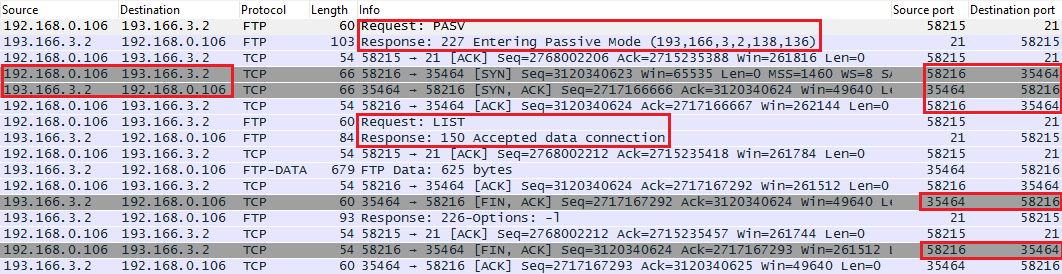
\includegraphics[scale = 0.60]{images/ftp16.png}
	
	\caption{Процесс передачи данных в пассивном режиме}
	\label{image:21}
\end{figure}

В первую очередь, клиент посылает на сервер (по управляющему каналу) команду PASV, в результате чего возвращается информация (IP + port) с кодом 227 (переход в пассивный режим) для последующего подключения канала данных. Затем, клиент инициирует установление соединения данных с произвольного порта на серверный порт, указанный в ответе на команду PASV ранее. Как только соединение данных установлено, на сервер отправляется команда LIST. Затем, клиенту отправляется сообщение с кодом 150 (подготавливается открытие канала), а также результат операции получения каталога. Финальным этапом является завершение соединения канала данных: клиенту отправляется сообщение с кодом 226 (закрытие канала, обмен завершен успешно), а канал данных обменивается флагами FIN и соединение завершается.

Стоит отметить, что в отличие от активного режима, установление соединения канала данных производится перед отправлением команды LIST по управляющему каналу.

Рассмотрим содержимое этих пакетов подробнее:

\begin{figure}[h!]
	\centering
	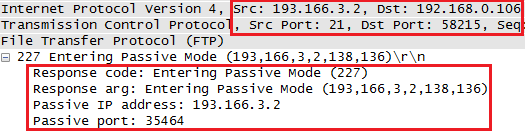
\includegraphics[scale = 0.75]{images/ftp17.png}
	
	\caption{Переход в пассивный режим}
	\label{image:22}
\end{figure}

\clearpage

\begin{figure}[h!]
	\centering
	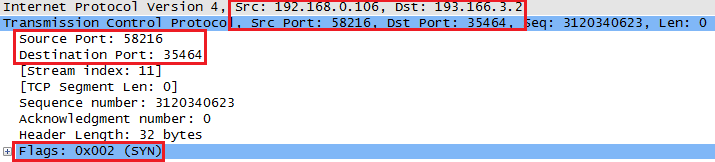
\includegraphics[scale = 0.75]{images/ftp18.png}
	
	\caption{Запрос на установление соединения данных от FTP клиента}
	\label{image:24}
\end{figure}


\begin{figure}[h!]
	\centering
	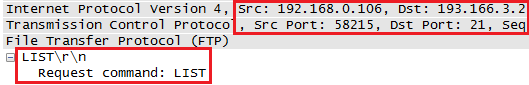
\includegraphics[scale = 0.75]{images/ftp19.png}
	
	\caption{Запрос на получение информации о каталоге}
	\label{image:23}
\end{figure}



\begin{figure}[h!]
	\centering
	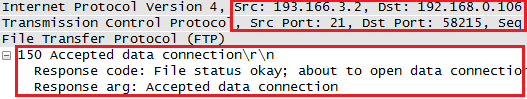
\includegraphics[scale = 0.75]{images/ftp20.png}
	
	\caption{Сообщение об успешном открытии канала данных}
	\label{image:25}
\end{figure}

\begin{figure}[h!]
	\centering
	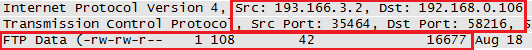
\includegraphics[scale = 0.75]{images/ftp21.png}
	
	\caption{Результат выполнения запрашиваемой команды}
	\label{image:26}
\end{figure}





\end{document}